\documentclass{report}
\usepackage{amsmath}
\usepackage{amsthm}
\usepackage{amssymb}
\usepackage{graphicx}

\usepackage[utf8]{inputenc}

\newtheorem{mydef}{Definition}
\newtheorem{myexample}{Beispiel}
\newtheorem{myproof}{Beweis}

\title{Grundlagen der Informatik}
\author{Simon Krenger, Gilles Bertholet}

\begin{document}
\maketitle
\chapter{Einführung}
\section{Lizenzen und Patente}
Unter einer Lizenz versteht man im rechtlichen Sinne ein \underline{Gebrauchsrecht}. Wenn Software gekauft wird, so wird das Gebrauchsrecht erworben. In der Informatik gibt es verschiedene Lizenzen, unter anderem folgende:
\begin{enumerate}
\item Open Source Lizenzen, z.B. die EULA: End User License Agreement
\item Closed Source Lizenzen, z.B. die GPL: GNU Public License (GNU = GNU Is Not Unix, $\to$ Richard Stallman)
\end{enumerate}

Konkret ist die Situation in der Schweiz irregulär.
\begin{quote}Legal, Illegal, Scheissegal\end{quote}
Lizenzen und Patente werden von der sogenannten "Intellectual Property (IP)" Lobby gfördert. Verfechter dieser Lobby werden mit den folgenden Begriffen in Verbindung gebracht:
\begin{enumerate}
\item Lizenzen
\item Patente
\item Trademarks (\texttrademark, entspricht in etwa \textregistered [= Registrierte Marke])
\end{enumerate}
Auf der anderen Seite haben wir die Bewegung der freien Software, die mit der GPL eine Lizenz erschaffen haben, welche die folgenden Eigenschaften besitzt (unvollständige Liste):
\begin{enumerate}
\item Enthält das Recht zum Kopieren
\item Enthält das Recht zu Reproduzieren
\item Neue Programme, die auf GPL Code basieren, müssen ebenfalls unter der GPL veröffentlicht werden.
\end{enumerate}
Als Konsequenz kann gesagt werden, dass es einen Gegensatz zwischen der "Open Source" Bewegung und der "Intellectual Property" Bewegung gibt.
\begin{center}Intellectual Property $\iff$ Open Source\end{center}
In der Schweiz gibt es keine Softwarepatente.
\begin{mydef}
Ein Patent ist ein hoheitlich erteiltes gewerbliches Schutzrecht für eine Erfindung. Der Inhaber des Patents ist berechtigt, anderen die Benutzung der Erfindung zu untersagen.
\end{mydef}
Ein Patent ist damit ein vom Staat erteiltes Monopol auf Bewirtschaftung eines Objektes (zeitlich begrenzt).
\begin{center}"Patente fördern Innovation" $\iff$ "Patente verhindern Innovation"\end{center}
Die Überlegungsweise bezüglich Lizenzierung hängt stark vom vertretenen Standpunkt aus. Unter einem \underline{Paradigmawechsel} versteht man einen Bruch in der Überlegungsweise.
\begin{myexample}Wir zeigen einen Paradigmawechsel anhand des Transportwesens vor und nach dem ersten Weltkrieg.
\begin{equation}\begin{tabular}{c | c}
Vor 1914 & Nach 1918\\
\hline
Pferde & Autos \\
Stroh & Tankstellennetzwerk\\
Stallknecht & Automechaniker \\
Sattler & Strassennetz \\
Schmied & Automechaniker\\
Kutscher & Fahrer\\
\end{tabular}\end{equation}\end{myexample}
In der Vergangenheit hat in der Informatik ein Paradigmawechsel vom Softwareverkauf hin zum Lizenzverkauf stattgefunden.
\begin{center}$\to$ Es werden keine Lösungen, sondern Lizenzen verkauft\end{center}
\section{Begriffe und Definitionen}
\subsection{Funktion / Struktur}
\begin{myexample}Wir erklären den Unterschied zwischen Funktion und Struktur anhand von zwei Beispielen.
\begin{enumerate}
\item Auto\\
Funktion: Mobilität\\
Struktur: Vier Räder, ein Motor, ein Steuerrad
\item Buch\\
Funktion: Informationsübermittlung\\
Struktur: Inhaltsverzeichnis, Prolog, Kapitel, Glossar\\
D.h. man erkennt auch bei einem chinesischen Buch eine Struktur, ohne den Inhalt zu verstehen.
\end{enumerate}
\end{myexample}
Durch eine sogenannte Strukturanalyse bei einem Codebeispiel wird nicht die Funktion ermittelt, sondern die Gesamtstruktur, die einzelnen Komponenten.
\begin{center}$\to$ Aufzählen der Komponenten\end{center}
\subsection{Analog / Digital}
\begin{center}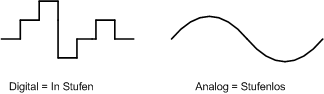
\includegraphics[scale=0.5]{img/analog-digital.png}\end{center}
Analog = Stufenlos\\
Digital = In Stufen / Zuständen\\
Wir haben die gleichen Konzepte in der Algebra: $\mathbb{R}$ ist nicht abzählbar, entspricht in etwa dem analogen Konzept. $\mathbb{N}$ und $\mathbb{Q}$ sind abzählbar, entsprechen daher eher dem digitalen Konzept.
\subsection{Daten / Informationen}
\begin{center}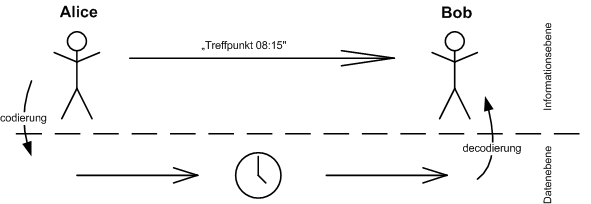
\includegraphics[scale=0.5]{img/daten-information.png}\end{center}
Daten sind lose vom Kontext, Informationen haben einen \underline{Kontext}. Man spricht davon, dass die Informationsebene kontextbehaftet ist. Reine Daten ohne Kontext können kaum interpretiert oder verarbeitet werden.
\subsection{Syntax / Semantik}
\begin{center}Syntax = Form $\iff$ Sinn = Semantik\end{center}
\begin{center}Syntax = Struktur $\iff$ Funktion = Semantik\end{center}
Ein Computer kann zwar die Syntax überprüfen, bei der Semantik (Sinn und Funktion des Programms) kann der Computer keine Überprüfung durchführen.
\section{Definition Computer}
Stichworte: "Rechner", "Hirn", "Input $\to$ Datenverarbeitung $\to$ Output"\\\\
Ein Computer ist ein abstrakter Begriff, wobei die konkrete Implementation auf verschiedene Arten passieren kann. Ein Computer kann analog oder digital sein, mechanisch, elektrisch oder biochemich realisiert sein.\\\\
Um den Computer zu definieren müssen wir eine Metabetrachtung (von aussen) durchführen. Bei einer Metabetrachtung wird ein formales System (System mit Regeln) extern und nicht von innen heraus betrachtet.\\\\
\underline{Alan Turing} (1912 - 1954) definiert einen Computer folgendermassen:
\begin{quote}Eine Maschine zur Manipulation von Zeichen\end{quote}
In der theoretischen Informatik unterscheidet man bei Programmiersprachen zwischen "turing-vollständigen" Sprachen und "nicht-turing-vollständigen" Sprachen. "Turing-vollständige" Sprachen können eine Turing-Maschine nachbilden. Wenn ein Problem in einer "turing-vollständigen" Sprache gelöst werden kann, so kann es in jeder anderen beliebig "turing-vollständigen" Sprache ebenfalls gelöst werden. Lediglich die Konzepte (z.B. Objektorientierung, Logische Programmierung, ...) ändern sich.
\section{Programiersprachen \& Algorithmen}
\begin{center}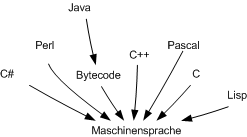
\includegraphics[scale=0.5]{img/hochsprachen.png}\end{center}
Hochsprachen nehmen dem Programmierer die trivialen Probleme ab (Speicherallozierung, Schleifen). Als Informatiker müssen wir die Konzepte hinter den Programmiersprachen verstehen. Dazu gehören neben der objektorientierten Programmierung beispielsweise die prozedurale oder logische Programmierung.\\\\
Es kann gesagt werden:
\begin{quote}Ein Algorithmus beschreibt einen Lösungsweg\end{quote}
\begin{quote}Ein Programm ist die Implementation eines Algorithmus\end{quote}
Bei der Implementation eines Algorithmus beschreibt die Programmiersprache die Regeln des formalen Systems.\\\\
Bei  der Programmierung wird im Grunde wie folgt vorgegangen:
\begin{quote}Problem $\to$ Metabetrachtung $\to$ Algorithmus $\to$ Lösung\end{quote}
Eine Metabetrachtung führen wir durch, in dem wir ausserhalb des Systems denken, am Besten mit einem Bleistift und einem Blatt Papier. Erst nach der Definition des Algorithmus können wir diesen in einem Programm am Computer umsetzen (Programmieren).\\\\
Ein Programm sollte sein:\begin{enumerate} 
\item \underline{Fehlerfrei}
\item \underline{Lesbar}
\item Kurz
\item Simpel
\item (Effizient)
\end{enumerate}
Laufzeiten lassen sich in verschiedene Komplexitätsklassen (vgl. Landau-Symbole) einteilen:
\begin{equation}O(c) \quad\mbox{= konstant}\end{equation}
\begin{equation}O(n) \quad\mbox{= linear}\end{equation}
\begin{equation}O(n^2) \quad\mbox{= quadratisch}\end{equation}
\begin{equation}O(2^n) \quad\mbox{= exponentiell}\end{equation}
\begin{equation}O(n log(n)) \quad\mbox{= logarithmisch}\end{equation}

\newpage
\section{Darstellung von Werten}
Es gibt verschiedene Möglichkeiten, Werte zu repräsentieren, so zum Beispiel:
\begin{quote}MDCVI $\to$ römisch 1606\end{quote}
\subsection{Dezimales Zahlensystem}
Das dezimale Zahlensystem ist ein System mit der Basis 10 und ist ein so genanntes positionelles System, d.h. die Position der Ziffer beeinflusst die repräsentierte Zahl.
\\\\Wir geben jeder Position einen Namen. Die Zahl 13408 besteht aus den folgenden Ziffern:
\begin{equation}\begin{tabular}{c c c c}
Ziffer & Position & Gewichtung & Exponent \\
\hline
1 & Zehntausender & 10000 & $10^4$ \\
3 & Tausender &  1000 & $10^3$ \\
4 & Hunderter & 100 & $10^2$ \\
0 & Zehner & 10 & $10^1$ \\
8 & Einer & 1 & $10^0$ \\
\end{tabular}\end{equation}
Wir sehen, dass die Zahl 13408 eigentlich die Summe aller Ziffern multipliziert mit ihrer Gewichtung ist. Konkret rechnen wir:
\begin{equation}1 \cdot 10000 + 3 \cdot 1000 + 4 \cdot 100 + 0 \cdot 10 + 8 \cdot 1\end{equation}
oder mit Exponentenschreibweise:
\begin{equation}1 \cdot 10^4 + 3 \cdot 10^3 + 4 \cdot 10^2 + 0 \cdot 10^1 + 8 \cdot 10^0\end{equation}
Der Exponent zeigt dabei die Position an (Position 0 bis Position 4). Allgemein formuliert:
\begin{eqnarray}&&a_n \cdot a_{n-1} \cdot a_{n-2} \cdot ... \cdot a_2 \cdot a_1 \cdot a_0 \nonumber \\
&=&a_n \cdot 10^n + a_{n-1} \cdot 10^{n-1} + ... + a_1 \cdot 10^1 + a_0 \cdot 10^0 \nonumber \\
&=&\sum_{i=0}^{n} a_i \cdot 10^i \quad \mbox{wobei}\quad a_i \in\ \{0, 1, 2, 3, ..., 8, 9\}\end{eqnarray}
Der Exponent $i$ enstspricht der Position im positionellen System, wird auch als Index bezeichnet.
Weiter halten wir fest:
\begin{quote}$a_n$ ist der Koeffizient\end{quote}
\begin{quote}$10$ ist die Basis\end{quote}
\begin{quote}$n$ ist der Index\end{quote}
Die einzelnen Ziffern der Ziffernmenge werden als \underline{Digits} bezeichnet.
\begin{equation}\mbox{Ziffernmenge} \quad a_i \in \{0, 1, 2, 3, ..., 8, 9\}\end{equation}
\subsection{Binäres Zahlensystem}
Im Gegensatz zum dezimalen Zahlensystem mit Basis 10 ändern wir beim binären Zahlensystem die Basis zu 2.
\begin{eqnarray}\mbox{Basis}:&\quad& 2 \nonumber \\
\mbox{Ziffernmenge}:&\quad&a_i \in \{0, 1\}\end{eqnarray}
Die einzelnen Ziffern der Ziffernmenge werden als \underline{Bits} bezeichnet.
\begin{eqnarray}&&a_n \cdot a_{n-1} \cdot a_{n-2} \cdot ... \cdot a_2 \cdot a_1 \cdot a_0 \nonumber \\
&=&a_n \cdot 2^n + a_{n-1} \cdot 2^{n-1} + ... + a_1 \cdot 2^1 + a_0 \cdot 2^0 \nonumber \\
&=&\sum_{i=0}^{n} a_i \cdot 2^i \quad \mbox{wobei}\quad a_i \in\ \{0, 1\}\end{eqnarray}
\begin{myexample}
\begin{eqnarray}1101_2&=&1 \cdot 2^3 + 1 \cdot 2^2 + 0 \cdot 2^1 + 1 \cdot 2^0 \nonumber \\
&=&8 + 4 + 0 + 1 \nonumber \\
&=&13\end{eqnarray}\end{myexample}
Zusätzlich definieren wir:
\begin{quote}8 Bit $\to$ 1 Byte\end{quote}
\begin{quote}4 Bit $\to$ 1 Nibble\end{quote}
\subsection{Hexadezimales System}
\begin{eqnarray}\mbox{Basis}:&\quad& 16 \nonumber \\
\mbox{Ziffernmenge}:&\quad&a_i \in \{0, 1, 2, ..., 8, 9, A, B, C, D, E, F\}\end{eqnarray}
\begin{eqnarray}&&a_n \cdot a_{n-1} \cdot a_{n-2} \cdot ... \cdot a_2 \cdot a_1 \cdot a_0 \nonumber \\
&=&a_n \cdot 16^n + a_{n-1} \cdot 16^{n-1} + ... + a_1 \cdot 16^1 + a_0 \cdot 16^0 \nonumber \\
&=&\sum_{i=0}^{n} a_i \cdot 16^i \quad \mbox{wobei}\quad a_i \in \{0, 1, 2, ..., D, E, F\}\end{eqnarray}
\begin{myexample}
\begin{eqnarray}A5_{16} = 0xA5&=&10 \cdot 16^1 + 5 \cdot 16^0 \nonumber \\
&=&165\end{eqnarray}\end{myexample}
\subsection{Umwandlung Hexadezimal und Binär}
Binäre Werte und hexadezimale Werte formen wir direkt um, analog folgender Tabelle:\begin{equation}\begin{tabular}{c | c | c}
Dezimal & Binär & Hexadezimal\\
\hline
0 & 0000 & 0x00\\
1 & 0001 & 0x01\\
2 & 0010 & 0x02\\
3 & 0011 & 0x03\\
4 & 0100 & 0x04\\
5 & 0101 & 0x05\\
6 & 0110 & 0x06\\
7 & 0111 & 0x07\\
8 & 1000 & 0x08\\
9 & 1001 & 0x09\\
10 & 1010 & 0x0A\\
11 & 1011 & 0x0B\\
12 & 1100 & 0x0C\\
13 & 1101 & 0x0D\\
14 & 1110 & 0x0E\\
15 & 1111 & 0x0F\\
\end{tabular}\end{equation}
\subsection{Umwandlung Basis n zu Basis 10}
Um eine Zahl mit einer beliebigen Basis $n$ umzurechnen, nutzen wir die Eigenschaften von positionellen Zahlensystemen.
\begin{eqnarray}\mbox{Basis}:&\quad& n \nonumber \\
\mbox{Ziffernmenge}:&\quad&a_i \in \mathbb{Z}_n\end{eqnarray}
\begin{eqnarray}&&a_m \cdot a_{m-1} \cdot a_{m-2} \cdot ... \cdot a_2 \cdot a_1 \cdot a_0 \nonumber \\
&=&a_m \cdot n^m + a_{m-1} \cdot n^{m-1} + ... + a_1 \cdot n^1 + a_0 \cdot n^0 \nonumber \\
&=&\sum_{i=0}^{m} a_i \cdot n^i \quad \mbox{wobei}\quad a_i \in\ \mathbb{Z}_n\end{eqnarray}
\subsection{Umwandlung Basis 10 zu Basis n}
Um eine Zahl von Basis 10 zu Basis N umzuwandeln, nutzen wir die Divisionsmethode (auch Modulo-Methode genannt). Dabei wird die umzuwandelnde Zahl im Dezimalsystem kontinuierlich mit der Basis dividieren. Wir zeigen dies anhand des folgenden Beispieles.
\begin{myexample}Wir wollen die Zahl $33_{10}$ als eine Zahl mit Basis $3$ schreiben.
\begin{eqnarray}
33 : 3 &=& 11 \quad \mbox{Rest} \quad 0 \nonumber \\
11 : 3 &=& 3 \quad \mbox{Rest} \quad 2 \nonumber \\
3 : 3 &=& 1 \quad \mbox{Rest} \quad 0 \nonumber \\
1 : 3 &=& 0 \quad \mbox{Rest} \quad 1\end{eqnarray}
Wir hören auf, sobald das Resultat 0 ergibt. Das Resultat lesen wir aus den Modulo-Werten von unten nach oben (in diesem Beispiel $33_{10} = 1020_3$).
\end{myexample}Wir dividieren die umzuwandelnde Zahl durch die zu erreichende Basis und schreiben den Rest in eine separate Spalte. Anschliessend wiederholen diese Schritte, bis wir als Resultat 0 erhalten.
\subsection{Umwandlung von Basis m zu Basis n}
Wir berechnen immer zuerst den Wert im Dezimalsystem und rechnen anschliessend mit der Divisionsmethode in die neue Basis um.
\begin{quote}Basis n $\to$ Basis 10 $\to$ Basis m\end{quote}
\newpage
\section{Darstellung von negativen Werten}
Im dezimalen System können wir eine Zahl mit dem Zeichen '-' negativ ausdrücken. Im binären System haben wir diese Möglichkeit nicht. Bis jetzt können wir nur die natürlichen Zahlen ($\mathbb{N}$) darstellen.
\subsection{Singed magnitude representation}
Wir stellen das Vorzeichen mit dem höchsten Bit (auch MSB, "most significant bit" genannt) dar und definieren:
\begin{equation}a_n \cdot a_{n-1} \cdot a_{n-2} \cdot ... \cdot a_1 \cdot a_0\end{equation}
wobei
\begin{eqnarray}a_n&=&Vorzeichen\nonumber \\
a_{n-1} \cdot a_{n-2} \cdot ... \cdot a_1 \cdot a_0 &=& Wert\end{eqnarray}
Dies führt uns allerdings zum Problem, dass einige Zahlen keine Eindeutige Zuordnung haben ($1000_2 = 0000_2 = 0$).
\subsection{Signed representation}
EIn Kilometerzähler mit 4 Stellen kann Zahlen von 0 bis 9999 darstellen, bei einem Überlauf (overflow) muss also sichergestellt werden, dass keine Information verloren geht. Um zu überprüfen, ob wir eine Zahl mit n Stellen darstellen können, brauchen wir den Modulo-Operator.
\begin{mydef}Wir definieren den Modulo wie folgt:\begin{equation}x \mod y := \mbox{Rest von} \quad\frac{x}{y}\end{equation}
Wir stellen dabei fest, dass der Modulo einer Zahl immer $< y$ ist.\end{mydef}
\begin{myexample}\begin{eqnarray}5 \mod 3 &=& 2\nonumber \\
4 \mod 3 &=& 1\nonumber \\
2 \mod 3 &=& 2\nonumber \\
1 \mod 3 &=& 1\nonumber \\
0 \mod 3 &=& 0\end{eqnarray}\end{myexample}Für das folgende Kapitel benötigen wir ausserdem die binäre Addition, welche wiederum den Modulo-Operator benötigt:
\begin{mydef}\begin{equation}a \oplus b := (a + b) \mod 2^n\end{equation}\end{mydef}
Wenn wir die Werte der Beispiele anschauen, bemerken wir, dass wir mit dem Zweier-Komplement negative Zahlen darstellen können, denn wenn wir den Algorithmus des Zweier-Komplements anwenden, so ergibt sich aus einer positiven Zahl deren negativer Wert und umgekehrt. Wir sehen dies auch anhand folgender Tabelle:
\begin{equation}\begin{tabular}{c c c}
Unsigned representation & & Signed representation \\
\hline
0 & 0000 & 0\\
1 & 0001 & 1\\
2 & 0010 & 2\\
3 & 0011 & 3\\
4 & 0100 & 4\\
5 & 0101 & 5\\
6 & 0110 & 6\\
7 & 0111 & 7\\
8 & 1000 & -8\\
9 & 1001 & -7\\
10 & 1010 & -6\\
11 & 1011 & -5\\
12 & 1100 & -4\\
13 & 1101 & -3\\
14 & 1110 & -2\\
15 & 1111 & -1\\ \end{tabular} \end{equation}
Den Schritt von 7 zu -8 nennen wir \underline{overflow}. Bei der unsigned representation nennen wir den Übergang von $1111_2$ zu $0000_2$ (Addition +1) \underline{carry}, da bei dieser Addition das Carry-Bit im Prozessor gesetzt wird.
\subsection{Vergleich signed, unsigned}
Wir sehen uns den Wertebereich der verschiedenen Darstellungen an, zuerst allgemein:
\begin{equation}\begin{tabular}{c | c c}
& signed representation & unsigned representation \\
\hline
Maximum & $2^{n-1}-1$ & $2^n-1$ \\
Minimum & $-(2^{n-1})$ & $0$\end{tabular}\end{equation}
Bei 4 Bits, bzw. bei 8 Bits:
\begin{equation}\begin{tabular}{c | c c}
4 Bits & signed representation & unsigned representation \\
\hline
Maximum & 7 & 15 \\
Minimum & -8 & 0\end{tabular}\end{equation}
\begin{equation}\begin{tabular}{c | c c}
8 Bits & signed representation & unsigned representation \\
\hline
Maximum & 127 & 255 \\
Minimum & -128 & 0\end{tabular}\end{equation}
\section{Binäre Operationen}
\subsection{Das Einer-Komplement K1 (Inversion)}
Das Einer-Komplement beschreibt die Inversion, also die Umkehrung der einzelnen Bits in einem binären Wert.
\begin{mydef}\begin{quote}$a_1 \in \{0, 1\}$\end{quote}\begin{eqnarray}
& &K1(a_n, \cdot a_{n-1}, \cdot a_{n-2} \cdot ... \cdot a_2 \cdot a_1 \cdot a_0) \nonumber \\
&:=& \lnot a_n, \cdot \lnot a_{n-1}, \cdot \lnot a_{n-2} \cdot ... \cdot \lnot a_2 \cdot \lnot a_1 \cdot \lnot a_0\end{eqnarray}\end{mydef}
\begin{myexample}$K1(1100) = 0011$\end{myexample}
\subsection{Das Zweier-Komplement K2 (Negation)}
WIr brauchen eine Methode, wie wir eine binäre Zahl darstellen können und diese einfach in eine negative Zahl konvertieren können. Dies machen wir mit dem Zweier-Komplement.
\begin{mydef}\begin{quote}$a_1 \in \{0, 1\}$\end{quote}\begin{eqnarray}
& &K2(a_n, \cdot a_{n-1}, \cdot a_{n-2} \cdot ... \cdot a_2 \cdot a_1 \cdot a_0) \nonumber \\
&=&K1(a_n, \cdot a_{n-1}, \cdot a_{n-2} \cdot ... \cdot a_2 \cdot a_1 \cdot a_0) \oplus 1 \end{eqnarray}\end{mydef}
\begin{myexample}\begin{eqnarray}K2(0110) &=& K1(0110) \oplus 1 \nonumber \\
&=&1001 \oplus 1 = (1001 + 0001) \mod 2^4 \nonumber \\
&=&1010_2 = 10_{10}\end{eqnarray}
\begin{eqnarray}K2(0000) &=& K1(0000) \oplus 1 \nonumber \\
&=&1111 \oplus 1 = (1111 + 0001) \mod 2^4 \nonumber \\
&=&10000 \mod 2^4 = 0000_2\end{eqnarray}
\begin{eqnarray}K2(1111) &=& K1(1111) \oplus 1 \nonumber \\
&=&0000 \oplus 1 = (0000 + 0001) \mod 2^4 \nonumber \\
&=&10001_2 = 1_{10}\end{eqnarray}
\begin{eqnarray}K2(0001) &=& K1(0001) \oplus 1 \nonumber \\
&=&1110 \oplus 1 = (1110 + 0001) \mod 2^4 \nonumber \\
&=&1111_2 = 15_{10}\end{eqnarray}\end{myexample}
\subsection{Addition}
Die binäre Addition beruht auf der folgenden Wahrheitswerttabelle, wenn wir zwei Bits $a_n$ und $b_n$ addieren:
\begin{center}\begin{tabular}{c c | c c}
$a_n$ & $b_n$ & Summe & $c_{n+1}$ \\ \hline
0 & 0 & 0 & 0 \\
0 & 1 & 1 & 0 \\
1 & 0 & 1 & 0 \\
1 & 1 & 0 & 1\end{tabular}\end{center}
Das Carry-Bit ($c_n$) wird dann zur nächsten Bit-Addition "mitgenommen". 
\begin{myexample}Wir zeigen die Addition an den folgenden Beispielen:
\begin{enumerate}
\item $6_{10}$ + $10_{10}$ = $16_{10}$\begin{center}\begin{tabular}{ccccccc}
& $0$ & $0$ & $0$ & $1$ & $1$ & $0$ \\
+ & $0$ & $0_1$ & $1_1$ & $0_1$ & $1$ & $0$ \\ \hline
& $0$ & $1$ & $0$ & $0$ & $0$ & $0$ \\ \hline \hline
\end{tabular}\end{center}
\end{enumerate}
\end{myexample}
\subsection{Subtraktion}
\begin{mydef}\begin{quote}$a - b := a \oplus K2(b)$\end{quote}\end{mydef}

\begin{myexample}\begin{tabular}{c c c c c}
\underline{unsigned} & & \underline{computer code} & & \underline{signed} \\
$\frac{12,15}{27}$ & $\leftarrow$ & $\begin{tabular}{c} 1000 \\ +1111 \\ \hline  0111  \\ \end{tabular} $ & $\overrightarrow{overflow}$ & $\begin{tabular}{c} -4 \\
+(-1) \\ \hline
-5 \\
\end{tabular} $ \\
$\not= 11$ & $\leftarrow$ & $\underline{0111} $ & $\rightarrow$ & $-5$ \\
\end{tabular}\end{myexample}
\section{Flags}
\subsection{Carry- und Overflowflag}
Um zu wissen, ob das angezeigte Resultat aus der vorhergegangenen Rechnung korrekt war, setzt der Prozessor sogenannte Flags. Hier soll nun das Carry-Flag und das Overflow-Flag besprochen werden.
\\\\
Das \underline{Carry-Flag} wird gesetzt, wenn das Resultat einer unsigned Rechnung nicht stimmt, d.h. wenn das korrekte Resultat grösser der maximal darstellbaren Zahl ist ($2^n-1$, wobei $n$ Anzahl der Bits ist) oder unter 0 fällt.
\\\\
Das \underline{Overflow-Flag} wird gesetzt, wenn bei einer arithmetischen Operation mit signed-Zahlen das Resultat entweder keiner der minimal darstellbaren Zahl ($< -(2^{n-1})$) ist oder grösser der maximal darstellbaren Zahl (> $2^{n-1}-1$) ist.

Allgemein stellen wir eine Addition wie folgt dar:
\begin{center}\begin{tabular}{ccccccc}
& $a_n$ & $a_{n-1}$ & $...$ & $a_2$ & $a_1$ & $a_0$ \\
+ & $b_n$ & $b_{n-1}$ & $...$ & $b_2$ & $b_1$ & $b_0$ \\ \hline
$c_{n+1}$ & $c_n$ & $c_{n-1}$ & $...$ & $c_2$ & $c_1$ & $c_0$
\end{tabular}\end{center}
Nun finden wir für das Carry-Flag, bzw. das Overflow-Flag folgende Regeln:
\begin{center}
\begin{tabular}{c|c|c|}
& Addition & Subtraktion \\ \hline
Carry-Flag & $C_{n+1}$ & $\lnot C_{n+1}$ \\ \hline
Overflow-Flag & \multicolumn{2}{|c|}{$(a_n \land b_n \land \lnot c_n) \lor (\lnot a \land \lnot b_n \land c_n)$} \\ \hline
\end{tabular}
\end{center}
Es ist wichtig zu verstehen, dass der Prozessor keinen Unterschied von unsigned und signed representation macht. Die Flags werden bei jeder Berechnung des Prozessors gesetzt. Das ausgeführte Programm muss dann die Flags beachten und entsprechend handhaben.
\chapter{Digitaltechnik}
Das \underline{Moorsche Gesetz} besagt, dass sich die Komplexität (= Anzahl Transistoren) integrierter Schaltkreise regelmässig verdoppelt. Je nach Quelle werden 18 oder 24 Monate als Zeitraum genannt.
\section{Produktion}
%TODO: Produktion
\section{Transistor}
%TODO: Einführung Transistor
\section{Gatter}
%TODO: Kurze Uebersicht zu den Gattern
\section{Flipflop}
%TODO: RS-Flipflop, Content: Schaltung, 
\section{Arithmetische Schaltungen}
\subsection{Halbaddierer}
% http://tams-www.informatik.uni-hamburg.de/applets/hades/webdemos/20-arithmetic/10adders/halfadd-fulladd.html
Ein Halbaddierer ist eine einfache logische Schaltung, mit welcher sich zwei Bits addieren lassen. Neben dem Resultat wird das Carry-Bit ausgegeben.
%TODO: BIld
\begin{center}\begin{tabular}{c c | c c}
$a_n$ & $b_n$ & Summe & $c_{n+1}$ \\ \hline
0 & 0 & 0 & 0 \\
0 & 1 & 1 & 0 \\
1 & 0 & 1 & 0 \\
1 & 1 & 0 & 1\end{tabular}\end{center}
Aus dieser Wahrheitswerttabelle können wir folgende boolsche Gleichungen herleiten:
\begin{eqnarray}
\mbox{Summe} & = & (a_n \land \lnot b_n) \lor (\lnot a \land b_n) \quad \mbox{(XOR)} \\
c_{n+1} & = & a_n \land b_n\end{eqnarray}
\subsection{Volladdierer}
% http://tams-www.informatik.uni-hamburg.de/applets/hades/webdemos/20-arithmetic/10-adders/halfadd-fulladd.html

Grundsätzlich handelt es sich beim Volladdierer um einen Halbaddierer, welcher das Carry-Bit der vorhergegangenen Addition ebenfalls in die Rechnung mit einbezieht. Statt zwei Eingänge haben wir nun drei Eingänge (nämlich $a$, $b$ und das Carry-Bit $c$).

%TODO: Bild
%TODO: Boolsche Gleichung
\begin{center}\begin{tabular}{c c c | c c}
$a_n$ & $b_n$ & $c_n$ & Summe & $c_{n+1}$ \\ \hline
0 & 0 & 0 & 0 & 0\\
0 & 0 & 1 & 1 & 0\\
0 & 1 & 0 & 1 & 0\\
0 & 1 & 1 & 0 & 1\\
1 & 0 & 0 & 1 & 0\\
1 & 0 & 1 & 0 & 1\\
1 & 1 & 0 & 0 & 1\\
1 & 1 & 1 & 1 & 1\\
\end{tabular}\end{center}
\subsection{Implementation Einfache ALU}
%TODO: http://tams-www.informatik.uni-hamburg.de/applets/hades/webdemos/20-arithmetic/40-addsub/add-sub.html
\section{Memory (Speicher)}
%TODO: Unterschied SRAM / DRAM
\subsection{Multiplexer}
Ein Multiplexer dient dazu, von einer beliebigen Anzahl Eingänge genau einen an den Ausgang weiter zu schalten. D.h. mittels der Addresseingänge können wir bestimmen, welcher Eingang an den Ausgang weitergegeben werden kann.
\subsection{Adress-Decoder}
Mit einem Adress-Decoder kann eine bestimmte Leitung am Adress-Decoder aktiv geschaltet werden. Über die Adresseingänge ($A_1 ... A_n$) können wir bestimmen, welcher Ausgang (bei 4 Adressbits $2^4$ = 16 Ausgänge) auf aktiv geschaltet wird.
\\\\
Im Folgenden die Wahrheitswerttabelle für einen 2:4 Adress-Decoder:
\begin{center}\begin{tabular}{c c | c c c c}
$A_1$ & $A_0$ & $O_3$ & $O_2$ & $O_1$ & $O_0$ \\ \hline
0 & 0 & 0 & 0 & 0 & 1\\
0 & 1 & 0 & 0 & 1 & 0\\
1 & 0 & 0 & 1 & 0 & 0\\
1 & 1 & 1 & 0 & 0 & 0\end{tabular}\end{center}
\subsection{Read Only Memory (ROM)}

\subsection{Random Access Memory (RAM)}

\end{document}